% Which components of COVER each ablation removes or replaces (Sec. 3, Ablations).
% Top: the components in data-flow order; below: one row per variant.
% Included with \includestandalone (sections/methodology.tex); also compiles alone.
\documentclass[tikz,border=3pt]{standalone}
\usepackage[T1]{fontenc}
\usepackage{newtxtext,newtxmath}
\usetikzlibrary{positioning,arrows.meta,calc}

% Same palette as cover_architecture.tex
\definecolor{neural}{HTML}{2F6DB5}
\definecolor{neuralbg}{HTML}{E8F0FA}
\definecolor{symb}{HTML}{D9822B}
\definecolor{symbbg}{HTML}{FCF0E3}
\definecolor{logic}{HTML}{2E8B57}
\definecolor{logicbg}{HTML}{E6F4EC}
\definecolor{relneg}{HTML}{C0392B}

\providecommand{\model}{COVER}
\providecommand{\cls}{\textsc{[cls]}}
\providecommand{\Pcov}{P_{\mathrm{cov}}}
\providecommand{\Pnc}{P_{\neg\mathrm{conf}}}

\tikzset{
  >={Stealth[length=1.6mm]},
  flow/.style={->, line width=0.6pt, draw=black!70},
  comp/.style={draw=#1, fill=#1bg, rounded corners=2.5pt, line width=0.7pt, minimum width=11.8mm,
               minimum height=10mm, align=center, font=\small, inner sep=1pt},
  keep/.style={fill=#1bg, draw=#1!70, rounded corners=1.5pt, minimum width=11.8mm, minimum height=4mm,
               inner sep=0pt, font=\footnotesize, text=#1!80!black},
  gone/.style={draw=black!25, dashed, rounded corners=1.5pt, minimum width=11.8mm, minimum height=4mm,
               inner sep=0pt, font=\footnotesize, text=relneg},
  rowlab/.style={anchor=east, font=\small, inner sep=1pt},
}

% column centres (cm)
\def\cE{2.25}\def\cL{3.55}\def\cG{4.85}\def\cS{6.15}\def\cC{7.45}\def\cA{9.05}
\def\dy{0.52}

% \K{x}{y}{colour}{text}: component kept; \X{x}{y}: removed; \XI{x}{y}: removed as a consequence
\newcommand{\K}[4]{\node[keep=#3] at (#1,#2) {#4};}
\newcommand{\KA}[2]{\node[keep=logic, minimum width=17mm] at (\cA,#1) {#2};}
\newcommand{\X}[2]{\node[gone] at (#1,#2) {$\times$};}
\newcommand{\XI}[2]{\node[gone, text=black!40] at (#1,#2) {$(\times)$};}

\begin{document}
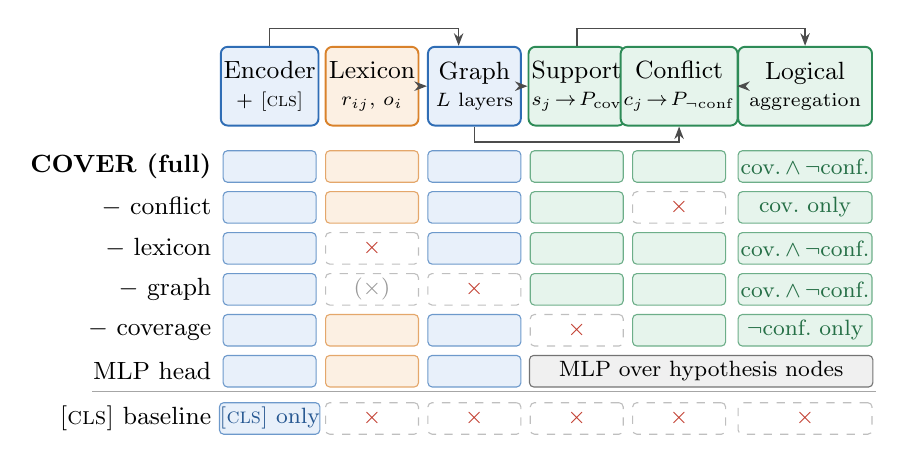
\begin{tikzpicture}

% ---------------------------------------------------------------- components
\node[comp=neural] (E) at (\cE,0) {Encoder\\[-1pt]{\scriptsize + \cls{}}};
\node[comp=symb]   (L) at (\cL,0) {Lexicon\\[-1pt]{\scriptsize $r_{ij},\,o_i$}};
\node[comp=neural] (G) at (\cG,0) {Graph\\[-1pt]{\scriptsize $L$ layers}};
\node[comp=logic]  (S) at (\cS,0) {Support\\[-1pt]{\scriptsize $s_j\!\to\!\Pcov$}};
\node[comp=logic]  (C) at (\cC,0) {Conflict\\[-1pt]{\scriptsize $c_j\!\to\!\Pnc$}};
\node[comp=logic, minimum width=17mm]  (A) at (\cA,0) {Logical\\[-1pt]{\scriptsize aggregation}};

\draw[flow] (L) -- (G);
\draw[flow] (E.north) -- ++(0,0.22) -| ([xshift=-2mm]G.north);
\draw[flow] (G) -- (S);
\draw[flow] (G.south) -- ++(0,-0.2) -| (C.south);
\draw[flow] (S.north) -- ++(0,0.22) -| (A.north);
\draw[flow] (C) -- (A);

% ---------------------------------------------------------------- variants
\def\y{-1.02}
\node[rowlab, font=\small\bfseries] at (1.55,\y) {\model{} (full)};
\K{\cE}{\y}{neural}{$\checkmark$}\K{\cL}{\y}{symb}{$\checkmark$}\K{\cG}{\y}{neural}{$\checkmark$}
\K{\cS}{\y}{logic}{$\checkmark$}\K{\cC}{\y}{logic}{$\checkmark$}\KA{\y}{cov.\,$\wedge$\,$\neg$conf.}

\pgfmathsetmacro{\y}{-1.02-\dy}
\node[rowlab] at (1.55,\y) {$-$ conflict};
\K{\cE}{\y}{neural}{$\checkmark$}\K{\cL}{\y}{symb}{$\checkmark$}\K{\cG}{\y}{neural}{$\checkmark$}
\K{\cS}{\y}{logic}{$\checkmark$}\X{\cC}{\y}\KA{\y}{cov.\ only}

\pgfmathsetmacro{\y}{-1.02-2*\dy}
\node[rowlab] at (1.55,\y) {$-$ lexicon};
\K{\cE}{\y}{neural}{$\checkmark$}\X{\cL}{\y}\K{\cG}{\y}{neural}{$\checkmark$}
\K{\cS}{\y}{logic}{$\checkmark$}\K{\cC}{\y}{logic}{$\checkmark$}\KA{\y}{cov.\,$\wedge$\,$\neg$conf.}

\pgfmathsetmacro{\y}{-1.02-3*\dy}
\node[rowlab] at (1.55,\y) {$-$ graph};
\K{\cE}{\y}{neural}{$\checkmark$}\XI{\cL}{\y}\X{\cG}{\y}
\K{\cS}{\y}{logic}{$\checkmark$}\K{\cC}{\y}{logic}{$\checkmark$}\KA{\y}{cov.\,$\wedge$\,$\neg$conf.}

\pgfmathsetmacro{\y}{-1.02-4*\dy}
\node[rowlab] at (1.55,\y) {$-$ coverage};
\K{\cE}{\y}{neural}{$\checkmark$}\K{\cL}{\y}{symb}{$\checkmark$}\K{\cG}{\y}{neural}{$\checkmark$}
\X{\cS}{\y}\K{\cC}{\y}{logic}{$\checkmark$}\KA{\y}{$\neg$conf.\ only}

\pgfmathsetmacro{\y}{-1.02-5*\dy}
\node[rowlab] at (1.55,\y) {MLP head};
\K{\cE}{\y}{neural}{$\checkmark$}\K{\cL}{\y}{symb}{$\checkmark$}\K{\cG}{\y}{neural}{$\checkmark$}
\node[draw=black!55, fill=black!6, rounded corners=1.5pt, minimum height=3.3mm, inner sep=0pt,
      font=\footnotesize, minimum height=4mm, minimum width=\cA cm-\cS cm+14.6mm] at ({(\cS+\cA+0.26)/2},\y)
      {MLP over hypothesis nodes};

\draw[black!35, line width=0.4pt] (0.0,{-1.02-5.5*\dy}) -- (9.95,{-1.02-5.5*\dy});

\pgfmathsetmacro{\y}{-1.02-6*\dy-0.08}
\node[rowlab] at (1.55,\y) {\cls{} baseline};
\K{\cE}{\y}{neural}{\cls{} only}\X{\cL}{\y}\X{\cG}{\y}\X{\cS}{\y}\X{\cC}{\y}\node[gone, minimum width=17mm] at (\cA,\y) {$\times$};

\end{tikzpicture}
\end{document}
